\chapter{DeepSeek}

\section{Multi-Head Latent Attention}

\begin{figure}[h]
	\centering
	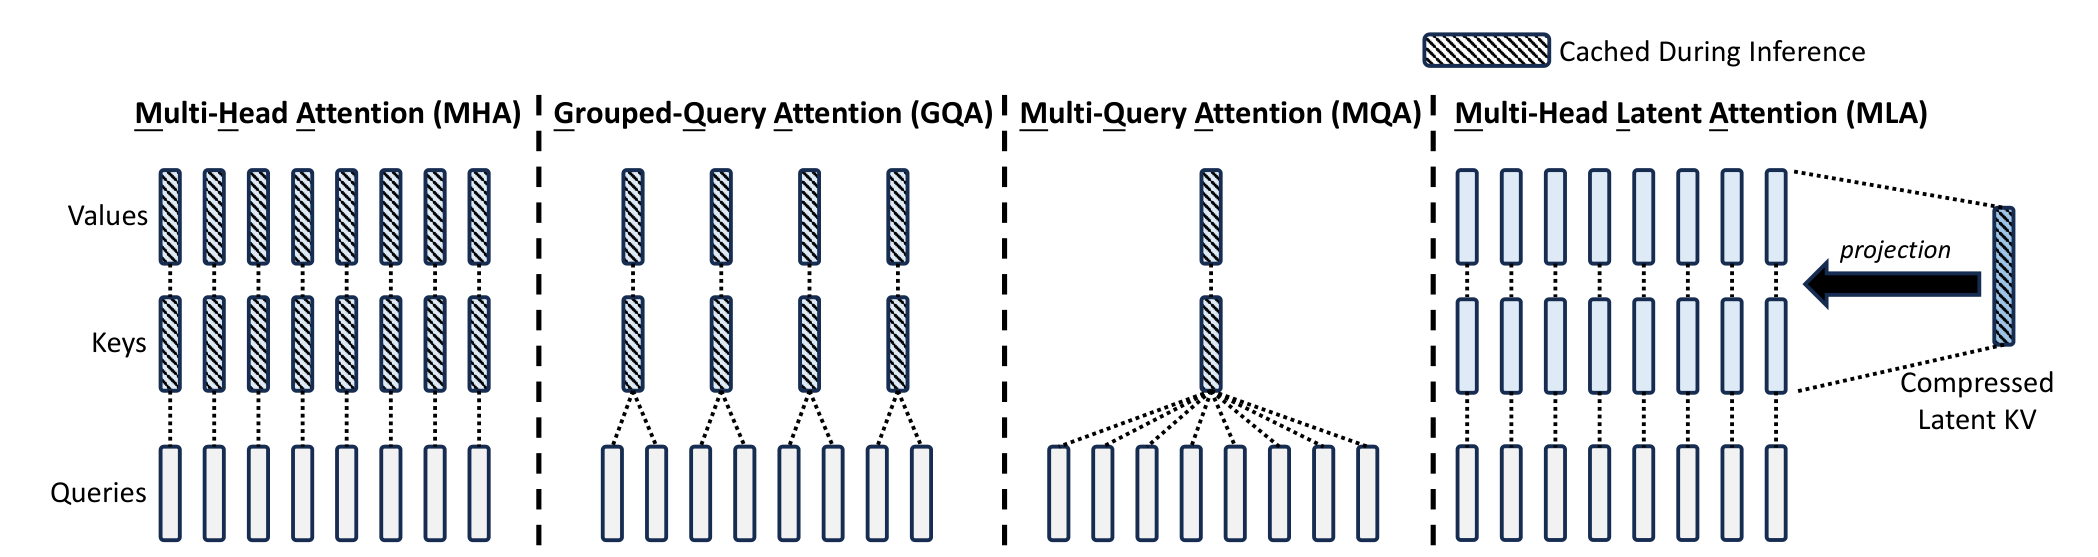
\includegraphics[scale=0.32]{./images/DeepSeek/mla.png}
\end{figure}

The query, key, and value of the vanilla multi-head attention can be expressed as follows:
\begin{align*}
	\rvq_t &= W^{Q}\rvh_t\\
	\rvk_t &= W^{K}\rvh_t\\
	\rvv_t &= W^{V}\rvh_t
\end{align*}
\begin{itemize}
	\item $\rvq_t,\rvk_t,\rvv_t\in \mathbb{R}^{d_hn_h}$
	\item $\rvh_t\in \mathbb{R}^{d}$: Attention input of the $t$-th token at an layer.
	\item $d_h$: the attention head's dimension
	\item $n_h$: the number of attention heads
\end{itemize}
During inference, all keys and values need to be cached to accelerate inference, so MHA needs to cache $2n_hd_hl$ elements (\ie key, value for each layer and head) for each token. In model deployment, this heavy KV cache is a large bottleneck that limits the maximum batch size and sequence length.

\begin{figure}[h]
	\centering
	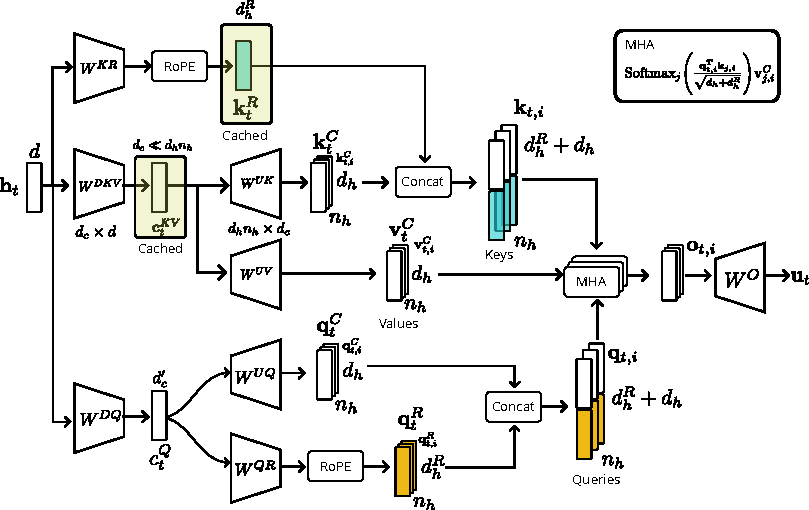
\includegraphics[scale=1.1]{./images/DeepSeek/mla.pdf}
	\caption{An overview of MLA.}
\end{figure}
In DeepSeek The key idea of Multi-Head Latent Attention (MLA) is the low-rank joint compression for attention keys and values to reduce Key-Value (KV) cache during inference:
\begin{align*}
	\rvc_t^{KV} &= W^{DKV}\rvh_t\\
	[\rvk_{t,1}^C; \rvk_{t,2}^C; \dots ;\rvk_{t,n_h}^C] = \rvk_t^{C} &= W^{UK}\rvc_t^{KV}\\
	\rvk_t^{R} &= \text{RoPE}(W^{KR}\rvh_t)\\
	\rvk_{t,i} &= [\rvk_{t,i}^C;\rvk_t^{R}]\\
	[\rvv_{t,1}^C; \rvv_{t,2}^C; \dots ;\rvv_{t,n_h}^C] = \rvv_t^{C} &= W^{UV}\rvc_t^{KV}
\end{align*}
\begin{itemize}
	\item $D$ and $U$ superscripts denote the up and down projection
	\item $\rvc_t^{KV}\in \mathbb{R}^{d_c}$ is the compressed (\ie $c$) \textit{latent vector} for keys and values, where $d_c\ll d_hn_h$. \textbf{Note that this is not a query vector.}
	\item $W^{DKV}\in \mathbb{R}^{d_c\times d}$ is the down-projection matrix
	\item $W^{UK},W^{UV}\in \mathbb{R}^{d_hn_h\times d_c}$ are the up-projection matrices for keys and values, respectively.
	\item $W^{KR}\in \mathbb{R}^{d_h^R\times d}$ is the matrix used for generating the decoupled key of RoPE. 
	\item \textbf{During inference, MLA only needs to cache $\rvc_t^{KV}$ and $\rvk_t^{R}$, which is a compressed latent vector, rather than high-dimensional key and value vector.} Thus, it can still have the multiple heads. This alleviates the issue of GQA or MQA while keeping their benefits. 
	\item Also, we do not have to explicitly compute the key and the values for attention.
		\begin{align*}
			q_t^Tk_t &= (W^{UQ}c_t^Q)^T(W^{UK}c_t^{KV})\\
					 &= (c_t^Q)^T(W^{UQT}W^{UK})c_t^{KV}
		\end{align*}
		\begin{itemize}
			\item Here, $W^{UQT}W^{UK}$ is a combined matrix of the projection matrices.
		\end{itemize}
		Similarly, for values,
		\begin{align*}
			o_{t,i} = \text{AttnScore}\cdot v_t^C
		\end{align*}
		The final output is
		\begin{align*}
			u_t &= W^O[o_{t,1}, \dots, o_{t,n_h}]\\
				&= W^O[\text{AttnScore}\cdot (W^{UV}c_t^{KV})]\\
				&= W^OW^{UV}[\text{AttnScore}\cdot (c_t^{KV})]
		\end{align*}
		\begin{itemize}
			\item To leverage this advantage, we need to use the \textit{decoupled RoPE}. Otherwise, the RoPE would be coupled with projection matrices.
		\end{itemize}
		\begin{align*}
			\rvq_t^T\rvk_t = (\rvc_t^Q)^T((W^{UQ})^TW^{UK})\rvc_T^{KV}
		\end{align*}
\end{itemize}

Moreover, in order to reduce the activation memory during training, we also perform low-rank compression for the queries, even if it cannot reduce the KV cache:
\begin{align*}
	\rvc_t^{Q} &= W^{DQ}\rvh_t\\
	[\rvq_{t,1}^C; \rvq_{t,2}^C; \dots ;\rvq_{t,n_h}^C] = \rvq_t^{C} &= W^{UQ}\rvc_t^{Q}\\
	[\rvq_{t,1}^R; \rvq_{t,2}^R; \dots ;\rvq_{t,n_h}^R] = \rvq_t^{R} &= \text{RoPE}(W^{QR}\rvc_t^Q)\\
	\rvq_{t,i} &= [\rvq_{t,i}^C;\rvq_{t,i}^{R}]
\end{align*}
\begin{itemize}
	\item $\rvc_t^{Q}\in \mathbb{R}^{d_c'}$ is the compressed latent vector for queries, where $d_c'\ll d_hn_h$
	\item $W^{DQ}\in \mathbb{R}^{d_c'\times d}$ and $W^{UQ}\in \mathbb{R}^{d_hn_h\times d_c'}$ are the down- and up- projection matrices for queries, respectively.
	\item $W^{QR}\in \mathbb{R}^{d_h^Rn_h\times d_c'}$ is the matrix for decoupled queries of RoPE.
\end{itemize}

Finally, the attention queries ($\rvq_{t,i}$), keys ($\rvk_{j,i}$), and values ($\rvv_{j,i}^C$) are combined to yield the final attention output $\rvu_t$:
\begin{align*}
	\rvo_{t,i} &= \sum_{j=1}^t\text{Softmax}_j\Bigg( \frac{\rvq_{t,i}^T\rvk_{j,i}}{\sqrt{d_h+d_h^R}} \Bigg)\rvv_{j,i}^C,\\
	\rvu_t &= W^O[\rvo_{t,1};\rvo_{t,2};\dots;\rvo_{t,n_h}],
\end{align*}
where $W^O\in \mathbb{R}^{d\times d_hn_h}$ is the output projection matrix.


\section{DeepSeek MoE}

\begin{figure}[t]
	\centering
	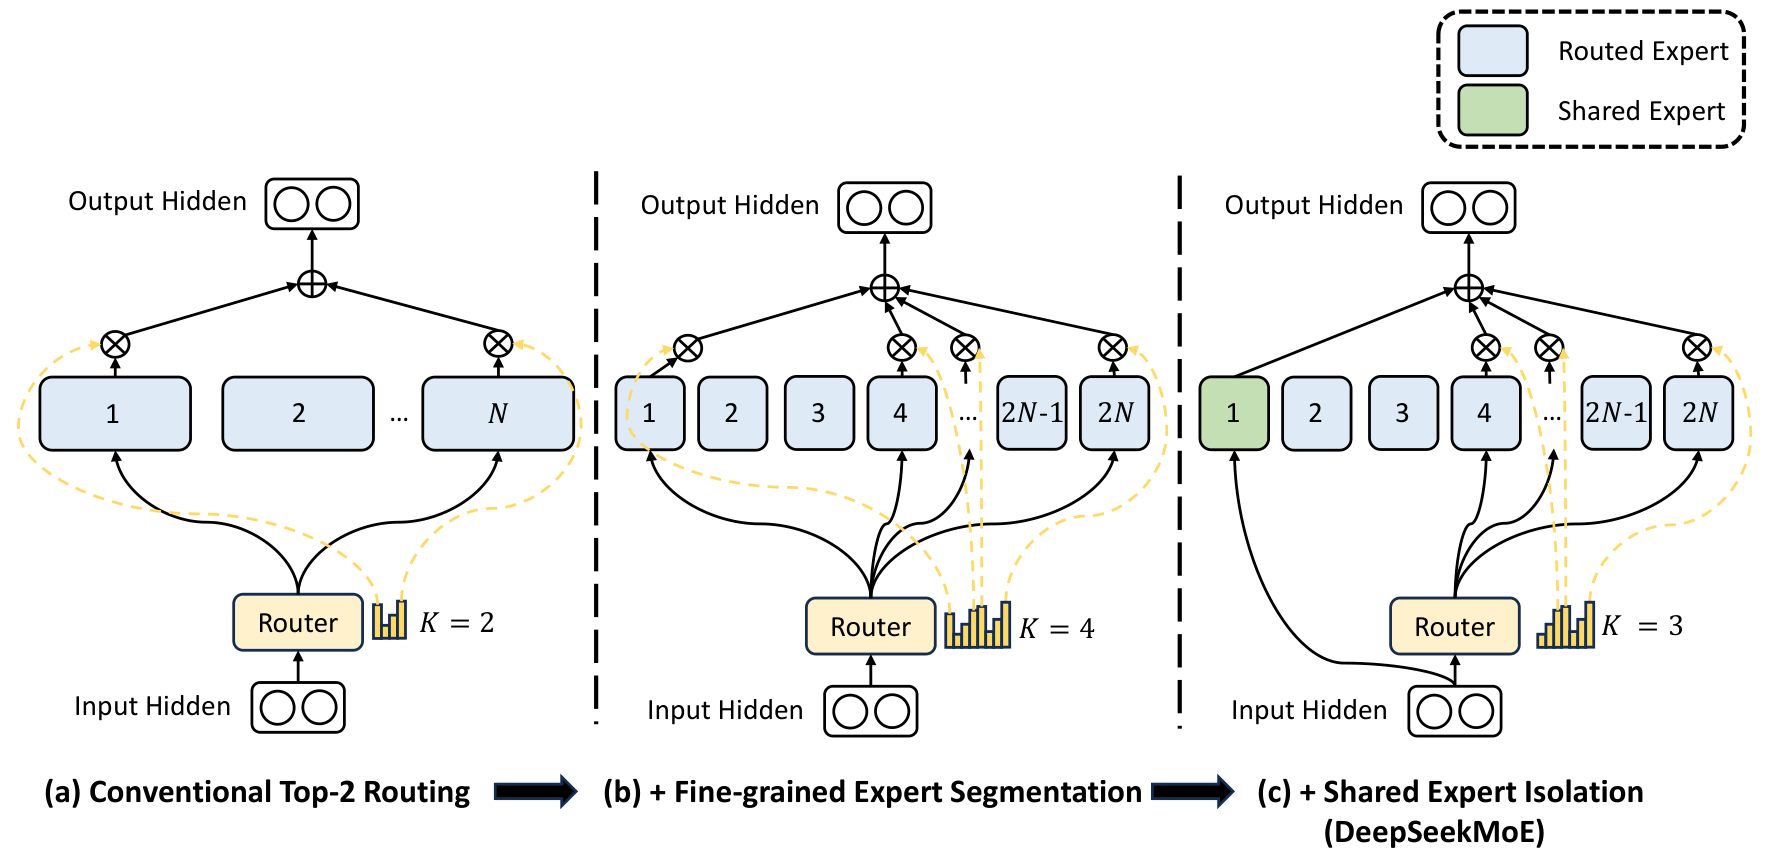
\includegraphics[scale=0.4]{./images/DeepSeek/deepseek_moe.png}
	\caption{An overview of DeepSeek MoE.}
	\label{fig:}
\end{figure}

This paper mentioned that the conventional TopK MoE has Knowledge Hybridity and Knowledge Redundancy. Knowledge Hybridity: existing MoE practices often employ a limited number of experts (e.g., 8 or 16), and thus tokens assigned to a specific expert will be likely to cover diverse knowledge. Consequently, the designated expert will intend to assemble vastly different types of knowledge in its parameters, which are hard to utilize simultaneously. (2) Knowledge Redundancy: tokens assigned to different experts may require common knowledge. As a result, multiple experts may converge in acquiring shared knowledge in their respective parameters, thereby leading to redundancy in expert parameters. These issues collectively hinder the expert specialization in existing MoE practices, preventing them from reaching the theoretical upper-bound performance of MoE models. By finely segmenting to more experts and introducing shared experts, DeepSeekMoE mitigated above two issues.

\begin{figure}[t]
	\centering
	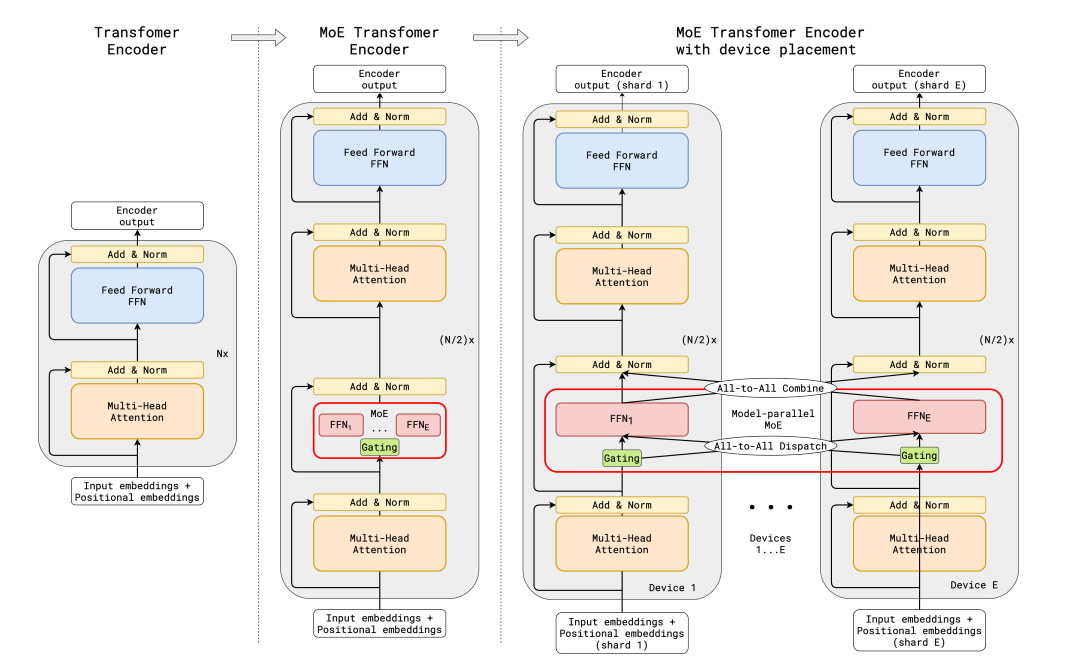
\includegraphics[scale=0.35]{./images/transformer/moe_block.png}
	\caption{MoE Transformer Encoder from the GShard Paper}
\end{figure}

A typical practice to construct an MoE language model usually substitutes FFNs in a Transformer with MoE layers at specified intervals. An MoE layer is composed of multiple experts, where each expert is structurally identical to a standard FFN. Then, each token will be assigned to one or two experts. If the 𝑙-th FFN is substituted with an MoE layer, the computation for its output hidden state h𝑙 𝑡is expressed as:
\begin{align*}
	\rvh_t' = \rvu_t+\sum^{N_s}_{i=1}FFN_i^{(s)}(\rvu_t)+\sum^{N_r}_{i=1}g_{i,t}FFN_i^{(r)}(\rvu_t),
\end{align*}
\begin{itemize}
	\item 
		\begin{align*}
			g_{i,t} = \frac{g_{i,t}'}{\sum^{N_r}_{j=1}g_{j,t}'},
		\end{align*}
		where
		\begin{align*}
			g_{i,t}' = \begin{cases}
				s_{i,t}&\text{ } s_{i,t}\in TopK(\{s_{j,t}|1\leq j \leq N_r\}, K_r)\\
				0&\text{otherwise,}
			\end{cases}
		\end{align*}
		$$s_{i,t} = \sigma(\rvu_t^T\rve_i)$$
	\item $\rvu_t$: FFN input of the $t$-th token. 
	\item $\rvh_t'$ FFN output
	\item $N_s$ and $N_r$ are the number of \textit{shared} experts and the \textit{routed} experts, respectively.
	\item $FFN_i^{(s)}(\cdot)$ and $FFN_i^{(r)}(\cdot)$ are the $i$-th \textit{shared} expert and the $i$-th \textit{routed} expert, respectively.
		\begin{itemize}
			\item The shared experts are always activated, aiming at capturing and consolidating common knowledge across varying contexts. 
			\item Through compressing common knowledge into these shared experts, redundancy among other routed experts will be mitigated.
		\end{itemize}
	\item $K_r$ is the number of activated routed experts
	\item $g_{i,t}$: gating value for the $i$-th expert, which is sparse by its nature. 
	\item $s_{i,t}$: a token assigned to an expert (\ie affinity score)
	\item $\rve_i$: the centroid vector of the $i$-th (routed) expert 
		\begin{itemize}
			\item This is an (learnable) expert embedding representing assignment scores for each token claimed by each expert. The shared expert would get a vector like $\mathbf{1}$, which is a vector of ones.
		\end{itemize}
	\item $TopK(\cdot, K)$: the set comprising $K$ highest scores among the affinity scores calculated for the $t$-th token and all routed experts.
	\item $\sigma$: Sigmoid function.
\end{itemize}

Let's closely look at the equation
\begin{align*}
	\rvh_t' = \rvu_t+\sum^{N_s}_{i=1}FFN_i^{(s)}(\rvu_t)+\sum^{N_r}_{i=1}g_{i,t}FFN_i^{(r)}(\rvu_t),
\end{align*}
\begin{itemize}
	\item $\rvu_t+\dots$: this is just a skip connection
	\item $\sum^{N_s}_{i=1}FFN_i^{(s)}(\rvu_t)$: Always activated
	\item $\sum^{N_r}_{i=1}g_{i,t}FFN_i^{(r)}(\rvu_t)$
		\begin{itemize}
			\item Here, we can notice that $g_{i,t}$ is the weight for the corresponding (routed) experts
		\end{itemize}
\end{itemize}

To balance the load of the experts, DeepSeek also introduces a bias term $b_i$ for each expert and add it to the corresponding scores $s_{i,t}$ as follows:
\begin{align*}
	g_{i,t}' = \begin{cases}
		s_{i,t}&\text{ } s_{i,t}+b_i\in TopK(\{s_{j,t}+b_i|1\leq j \leq N_r\}, K_r)\\
		0&\text{otherwise,}
	\end{cases}
\end{align*}
During training, the bias term decreases by $\gamma$ at the end of each step if its corresponding expert is overloaded. 


\section{Multi-Token Prediction}

DeepSeek also adopts a multi-token prediction approach and they show that it can improve the output quality and generalization behaviors. One of potential reasons would be that MTP may mitigate the distributional discrepancy between training time teacher forcing and inference time autoregressive generation.

Unlike the conventional MTP approach, they keep the complete causal chain at each prediction depth by introducing MTP modules.

The input tokens $[t_1,t_2,t_3,t_4]$ go through the main model's transformer blocks and then go through the output head of main model to produce next predicted token $t_5$. Meanwhile the representation of the input tokens $[t_1,t_2,t_3,t_4]$ (\ie output of main model's transformer blocks) will be passed to the MTP module and combine them with new input tokens' embedding$[t_2,t_3,t_4,t_5]$ to help produce additional token $t_6$. In DeepSeek-V3, the model is designed to predict next 2 tokens.

\begin{align*}
	\rvh_i^{'k} = M_k[\text{RMSNorm}(\rvh_i^{k-1}); \text{RMSNorm}(\text{Emb}(t_{i+k}))]
\end{align*}
\begin{itemize}
	\item $\rvh_i^{k-1}$: $i$-th token at the $(k-1)$-th depth 
	\item $(i+k)$-th token embedding $\text{Emb}(t_{i+k})$
\end{itemize}

\section{Reinforcement Learning}
\subsection{Backgrounds: Proximal Policy Optimization}
The objective function of Proximal Policy Optimization (PPO) can be represented as follows:
\begin{align*}
	\theta_{k+1} = \underset{\theta}{\operatorname{argmax}} \underset{s,a\sim \pi_{\theta_k}}{\mathbb{E}} [L(s, a, \theta_k, \theta)],
\end{align*}
where $\theta_{k}$ is a parameter of a policy network at $k$-th step, $\theta$ is the current policy we want to update, and the $A$ is the advantage (\ie reward). Finally, the $L$ is given by
$$L(s, a, \theta_k, \theta) = \min \Bigg(\frac{\pi_{\theta}\left(a | s\right)}{\pi_{\theta_{\text {k}}}\left(a | s\right)} A^{\pi_{\theta_k}}(s,a), \textrm{ Clip}\Bigg(\frac{\pi_{\theta}\left(a | s\right)}{\pi_{\theta_{\text {k}}}\left(a | s\right)}, 1-\varepsilon, 1+\varepsilon\Bigg) A^{\pi_{\theta_k}}(s,a)\Bigg).$$
Roughly, $\varepsilon$ is a hyperparameter which says how far away the new policy is allowed to go from the old one. A simpler expression of the above expression is
\begin{align}
	L(s, a, \theta_k, \theta) = \min \Bigg(\frac{\pi_{\theta}\left(a | s\right)}{\pi_{\theta_{\text {k}}}\left(a | s\right)} A^{\pi_{\theta_k}}(s,a), g(\varepsilon, A^{\pi_{\theta_k}}(s,a)) \Bigg),
	\label{eq:ppo_objective}
\end{align}
where 
\begin{align}
	g(\varepsilon,A) = 
	\begin{cases}
		(1+\varepsilon)A & A\geq 0\\
		(1-\varepsilon)A & A< 0.
	\end{cases}
	\label{eq:ppo_clip}
\end{align}

\begin{enumerate}
	\item Positive Advantage: Suppose the advantage for that state-action pair is positive, in which case its contribution to the objective reduces to
\begin{align}
	L(s, a, \theta_k, \theta) = \min \Bigg(\frac{\pi_{\theta}\left(a | s\right)}{\pi_{\theta_{\text {k}}}\left(a | s\right)}, 1+\varepsilon \Bigg) A^{\pi_{\theta_k}}(s,a).
	\label{eq:ppo_positive}
\end{align}
As the advantage is positive, the objective will increase if the action becomes more likely that is, if $\pi_{\theta}(a|s)$ increases. But the min in this term puts a limit to how much the objective can increase. Once $\pi_{\theta}(a|s) > (1+\epsilon) \pi_{\theta_k}(a|s)$, the min kicks in and this term hits a ceiling of $(1+\epsilon) A^{\pi_{\theta_k}}(s,a)$. Thus, the new policy does not benefit by going far away from the old policy.
\item Negative Advantage: Suppose the advantage for that state-action pair is negative, in which case its contribution to the objective reduces to
\begin{align}
	L(s, a, \theta_k, \theta) = \max \Bigg(\frac{\pi_{\theta}\left(a | s\right)}{\pi_{\theta_{\text {k}}}\left(a | s\right)}, 1-\varepsilon \Bigg) A^{\pi_{\theta_k}}(s,a).
	\label{eq:ppo_negative}
\end{align}
Since the advantage is negative, the objective will increase if the action becomes less likely. In other words, if $\pi_{\theta}(a|s)$ decreases. But the max in this term puts a limit to how much the objective can increase. Once $\pi_{\theta}(a|s) < (1-\epsilon) \pi_{\theta_k}(a|s)$, the max kicks in and this term hits a ceiling of $(1-\epsilon) A^{\pi_{\theta_k}}(s,a)$. Thus, again, the new policy does not benefit by going far away from the old policy.
\end{enumerate}
In sum, \textbf{clipping serves as a regularizer} by restricting the rewards to the policy, which change it dramatically with the hyperparameter $\epsilon$ corresponds to how far away the new policy can go from the old while still profiting the objective.

\subsection{Group Relative Policy Optimization}

\begin{figure}[t]
	\centering
	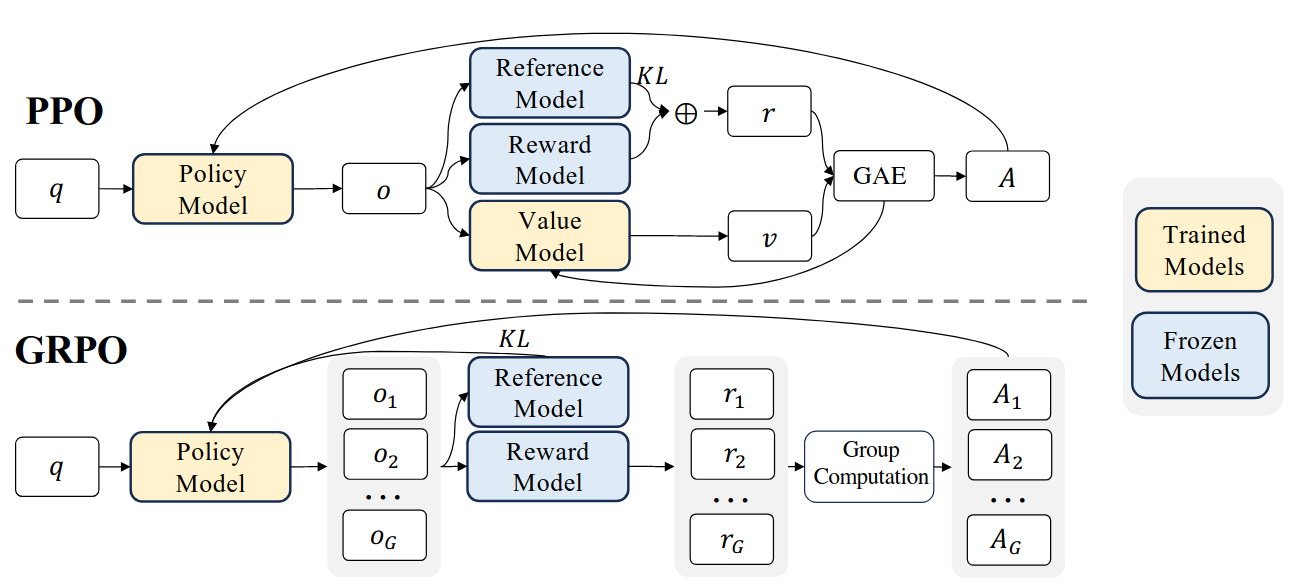
\includegraphics[scale=0.5]{./images/DeepSeek/grpo.png}
	\caption{An illustration of GRPO. The policy model $\pi$ takes an question (\ie observation, $q$) and generates answers (\ie actions, $o_1$) of the question. }
\end{figure}

Similarly, in DeepSeek, they leveraged a RL objective called Group Relative Policy Optimization (GRPO), which is a variant of PPO. 
\begin{align*}
	\mathcal{J} = \frac{1}{G}\sum_{i=1}^{G} \min \Bigg(\frac{\pi_{\theta}\left(o_i | q\right)}{\pi_{\theta_{\text {k}}}\left(o_i | q\right)} A_i, \textrm{ Clip}\Bigg(\frac{\pi_{\theta}\left(o_i | q\right)}{\pi_{\theta_{\text {k}}}\left(o_i | q\right)}, 1-\varepsilon, 1+\varepsilon\Bigg) A_{i}\Bigg) -\beta D_{KL}(\pi_{\theta}\| \pi_{\text{ref}}).
\end{align*}
\begin{itemize}
	\item GRPO samples a group of outputs $\{o_1, o_2,\dots, o_G \}$ from the old policy $\pi_{\theta_k}$ and then optimizes the policy model by maximizing the objective 
	\item The KL-divergence is used to restrict the sudden change of policy.
	\item The advantage can be calculated by averaging and normalizing the rewards.
	\item Instead of using a value model explicitly, GRPO computes a value of the states (\ie $o_i$) by averaging them. 
		\begin{itemize}
			\item $A(s,a) = Q(s,a)-V(s)$
		\end{itemize}
	\item $\pi_{\text{ref}}$ is the reference model, which is an initial SFT model. 
\end{itemize}

% \section{Training FrameWork}
% \begin{itemize}
% 	\item 2048 H800 GPUs
% 	\item HAI-LLM framework: their custom framework. 
% 	\item 16-way Pipeline Parallelism
% 		\begin{itemize}
% 			\item The layers of a model are sharded across multiple devices. 
% 		\end{itemize}
% 	\item Expert Parallelism: evenly distributes some of the experts' full weight to different GPUs, which means each GPU holds part of the experts' full weight. \eg experts 1, 2, and 3 are assigned to the first GPU, while experts 4, 5, and 6 are assigned to the second one.
% 	\item ZeRO-1 DP
% \end{itemize}
% \section{DualPipe}
% \section{FP8}

\section{DeepSeek-R1}

\begin{itemize}
	\item DeepSeek-R1-Zero, which applies RL directly to the base model without any SFT data, 
	\item DeepSeek-R1, which applies RL starting from a checkpoint fine-tuned with thousands of long Chain-of-Thought (CoT) examples. 
	\item Distill the reasoning capability from DeepSeek-R1 to small dense models.
\end{itemize}

\subsection{DeepSeek-R1-Zero}
The reward is the source of the training signal, which decides the optimization direction of RL. To train DeepSeek-R1-Zero, we adopt a rule-based reward system that mainly consists of two types of rewards:

\begin{itemize}
	\item Accuracy rewards: The accuracy reward model evaluates whether the response is correct. For example, in the case of math problems with deterministic results, the model is required to provide the final answer in a specified format (\eg within a box), enabling reliable rule-based verification of correctness. Similarly, for LeetCode problems, a compiler can be used to generate feedback based on predefined test cases. 
	\item Format rewards: In addition to the accuracy reward model, we employ a format reward model that enforces the model to put its thinking process between <think> and </think> tags.
\end{itemize}

Note that \textit{R1 does not use a neural reward model.}

Aha Moment of DeepSeek-R1-Zero A particularly intriguing phenomenon observed during the training of DeepSeek-R1-Zero is the occurrence of an aha moment. This moment, as illustrated in Table 3, occurs in an intermediate version of the model. During this phase, \textbf{DeepSeek-R1-Zero learns to allocate more thinking time to a problem by reevaluating its initial approach.} This behavior is not only a testament to the model's growing reasoning abilities but also a captivating example of how reinforcement learning can lead to unexpected and sophisticated outcomes.

This moment is not only an aha moment for the model but also for the researchers observing its behavior. It underscores the power and beauty of reinforcement learning: rather than explicitly teaching the model on how to solve a problem, we simply provide it with the right incentives, and it autonomously develops advanced problem-solving strategies. The aha moment serves as a powerful reminder of the potential of RL to unlock new levels of intelligence in artificial systems, paving the way for more autonomous and adaptive models in the future.

\begin{figure}[t]
	\centering
	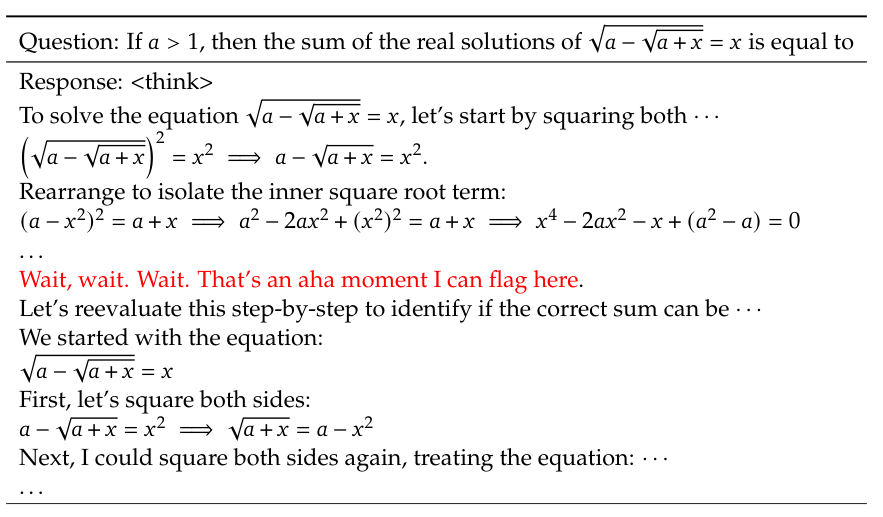
\includegraphics[scale=0.5]{./images/DeepSeek/aha_moment.png}
\end{figure}

\subsection{DeepSeek-R1}
We construct and collect a small amount of long CoT data (thousands) to fine-tune the model as the initial RL actor.

\begin{itemize}
	\item A key limitation of DeepSeek-R1-Zero is that its content is often not suitable for reading
	\item In contrast, when creating cold-start data for DeepSeek-R1, we design a readable pattern that includes a summary at the end of each response and filters out responses that are not reader-friendly. Here, we define the output format as |special-token|<reasoning-process>|special-token|<summary>, where the reasoning process is the CoT for the query, and the summary is used to summarize the reasoning results.
\end{itemize}

When reasoning-oriented RL converges, we utilize the resulting checkpoint to collect SFT (Supervised Fine-Tuning) data for the subsequent round. Unlike the initial cold-start data, which primarily focuses on reasoning, this stage incorporates data from other domains to enhance the model's capabilities in writing, role-playing, and other general-purpose tasks. Specifically, we generate the data and fine-tune the model as described below.

We curate reasoning prompts and generate reasoning trajectories by performing rejection sampling from the checkpoint from the above RL training. In the previous stage, we only included data that could be evaluated using rule-based rewards. However, in this stage, we expand the dataset by incorporating additional data, some of which use a generative reward model by feeding the ground-truth and model predictions into DeepSeek-V3 for judgment. Additionally, because the model output is sometimes chaotic and difficult to read, we have filtered out chain-of-thought with mixed languages, long parapraphs, and code blocks. For each prompt, we sample multiple responses and retain only the correct ones. In total, we collect about 600k reasoning related training samples.

To equip more efficient smaller models with reasoning capabilities like DeepSeek-R1, we directly fine-tuned open-source models like Qwen (Qwen, 2024b) and Llama (AI@Meta, 2024) using the 800k samples curated with DeepSeek-R1.
